\chapter{计算机网络}

\section{概述}


\subsection{计算机网络的作用}

计算机网络,是指将地理位置不同的具有独立功能的多台计算机,通过通信线路连接起来,在网络通信协议的管理和协调下,实现\textbf{信息交换和资源共享}的计算机系统。


\begin{description}
  \item[信息交换] 计算机网络使上网用户之间都可以进行信息交互,好像这些用户的计算机都可以彼此直接连通一样。
  \item[资源共享] 可以是信息共享、软件共享,也可以是硬件共享。
\end{description}



\subsection{因特网概述}

因特网起源于美国,现已发展成为世界上最大的国际性计算机互联网。网络(network)由若干结点(node)和连接这些结点的链路(link) 组成。互联网是“网络的网络”(network of networks)。连接在因特网上的计算机都称为主机(host)。

网络把许多计算机连接在一起,因特网则把许多网络连接在一起,如图所示。

\begin{figure}
  \centering
  % Requires \usepackage{graphicx}
  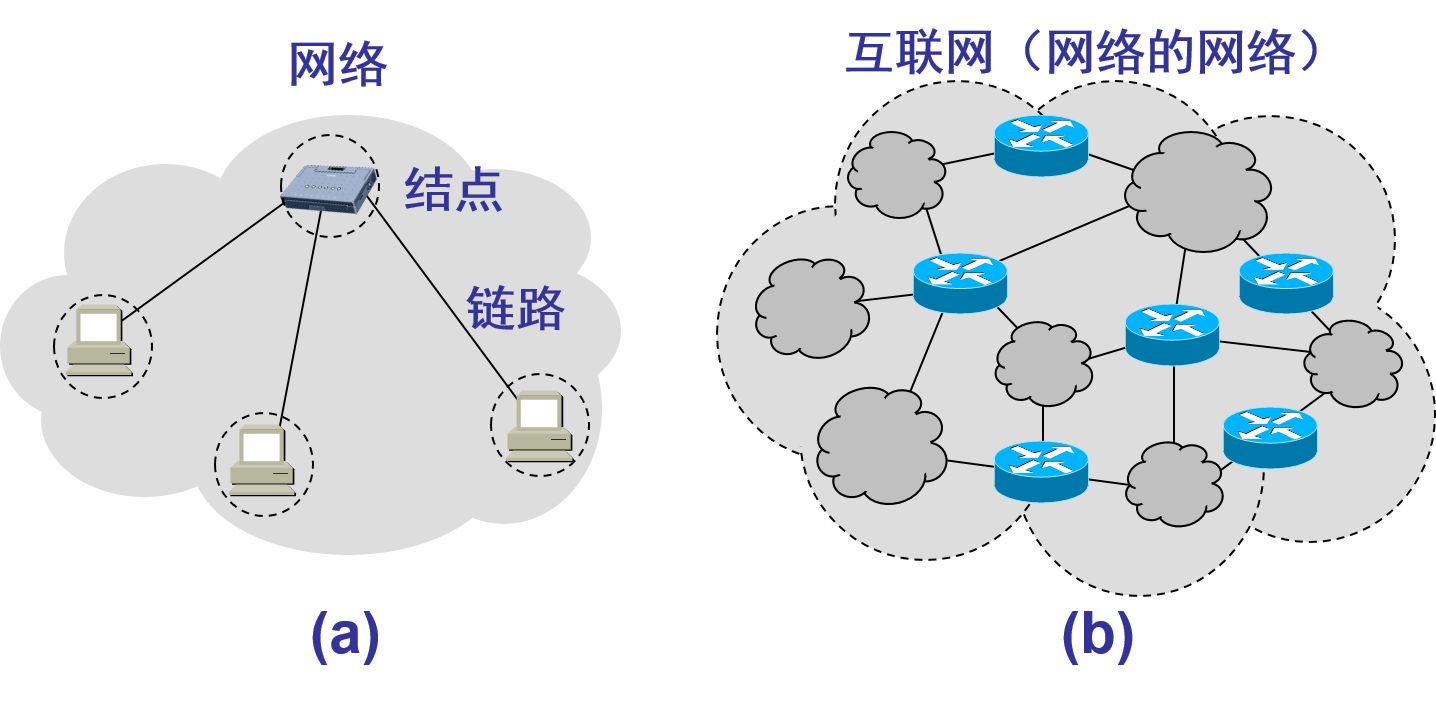
\includegraphics[width=0.55\textwidth]{fig_7_01}
  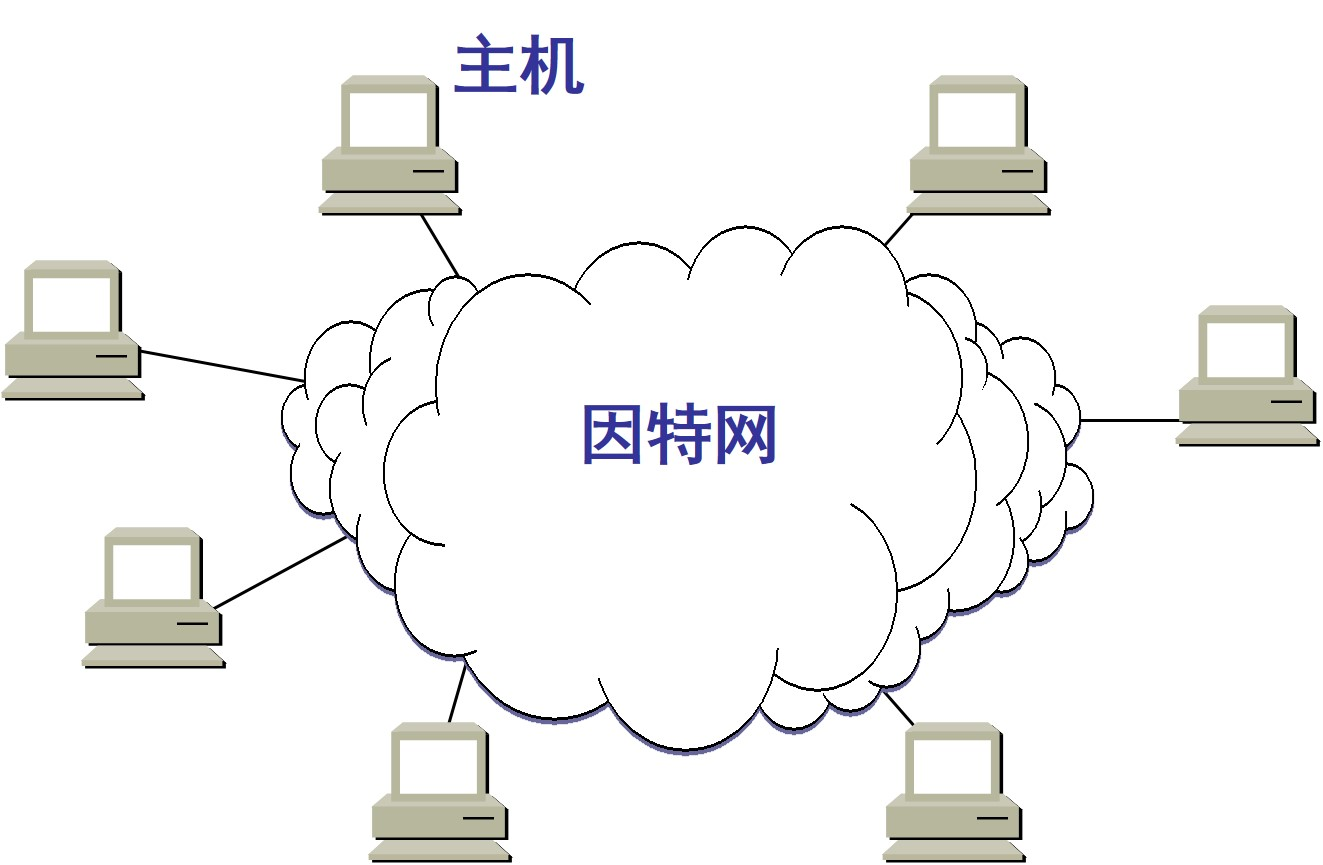
\includegraphics[width=0.4\textwidth]{fig_7_01a}\\
  \caption{网络的网络-互联网}\label{fig_7_01}
\end{figure}


因特网发展的三个阶段:
\begin{enumerate}
  \item 第一阶段(1969-1983):单个网络 ARPANET向互联网发展的过程。

  \item 第二阶段(1983-1995):该阶段的特点是建成了三级结构(主干网、地区网和校园网)的因特网。


  \item 第三阶段(1995-至今):该阶段的特点是逐渐形成了多层次 ISP 结构的因特网。出现了因特网服务提供者 ISP (Internet Service Provider)。
\end{enumerate}


\subsection{因特网的组成}

如图所示,从因特网的工作方式上看,可以划分为以下的两大块:
\begin{enumerate}
  \item \textbf{边缘部分}

  由所有连接在因特网上的主机组成。这部分是用户直接使用的,用来进行通信(传送数据、音频或视频)和资源共享。
  \item \textbf{核心部分}

  由大量网络和连接这些网络的路由器组成。这部分是为边缘部分提供服务的(提供连通性和交换)。
\end{enumerate}

\begin{figure}
  \centering
  % Requires \usepackage{graphicx}
  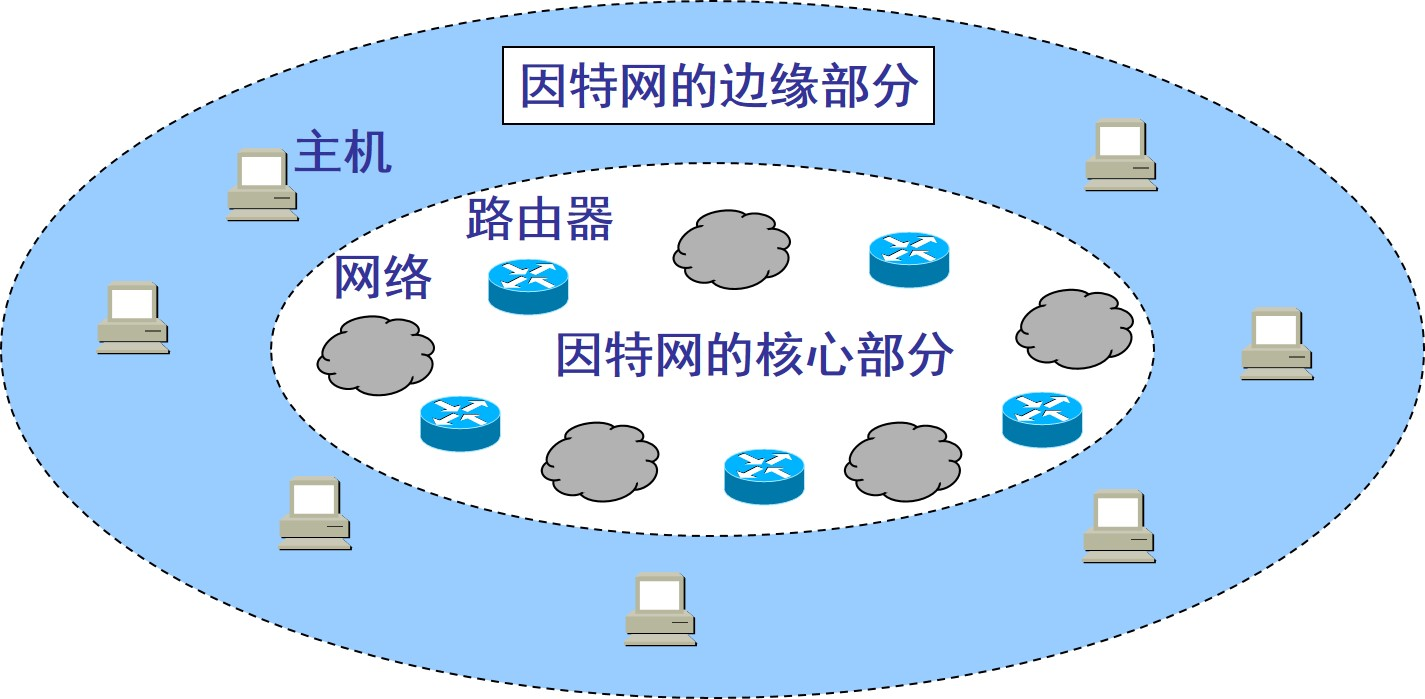
\includegraphics[width=0.5\textwidth]{fig_7_02}
  \caption{因特网的边缘部分与核心部分}\label{fig_7_02}
\end{figure}



\subsection{边缘部分}

处在因特网边缘的部分就是连接在因特网上的所有的主机,又称为端系统。 “主机 A 和主机 B 进行通信”,实际上是指:“运行在主机 A 上的某个程序和运行在主机 B 上的另一个程序进行通信”。即“主机 A 的某个进程和主机 B 上的另一个进程进行通信”。或简称为“计算机之间通信”。如图\ref{fig_7_03}所示,在网络边缘的端系统中运行的程序之间的通信方式通常可划分为两大类:

\begin{enumerate}
  \item 客户/服务器方式(C/S 方式):Client/Server方式
  \begin{itemize}
    \item 客户(client)和服务器(server)都是指通信中所涉及的两个应用进程。

\item 客户服务器方式所描述的是进程之间服务和被服务的关系。

\item 客户是服务的请求方,服务器是服务的提供方。

\item 客户软件的特点:

被用户调用后运行,在打算通信时主动向远地服务器发起通信(请求服务)。因此,客户程序必须知道服务器程序的地址。不需要特殊的硬件和很复杂的操作系统。

\item 服务器软件的特点:

一种专门用来提供某种服务的程序,可同时处理多个远地或本地客户的请求。
系统启动后即自动调用并一直不断地运行着,被动地等待并接受来自各地的客户的通信请求。因此,服务器程序不需要知道客户程序的地址。
一般需要强大的硬件和高级的操作系统支持。



  \end{itemize}
  \item 对等方式(P2P 方式):即 Peer-to-Peer方式


  \begin{itemize}
    \item 对等连接(peer-to-peer,简写为 P2P)是指两个主机在通信时并不区分哪一个是服务请求方还是服务提供方。

\item 只要两个主机都运行了对等连接软件( P2P 软件),它们就可以进行平等的、对等连接通信。
\item 双方都可以下载对方已经存储在硬盘中的共享文档。

  \end{itemize}
\end{enumerate}



\begin{figure}
  \centering
  % Requires \usepackage{graphicx}
  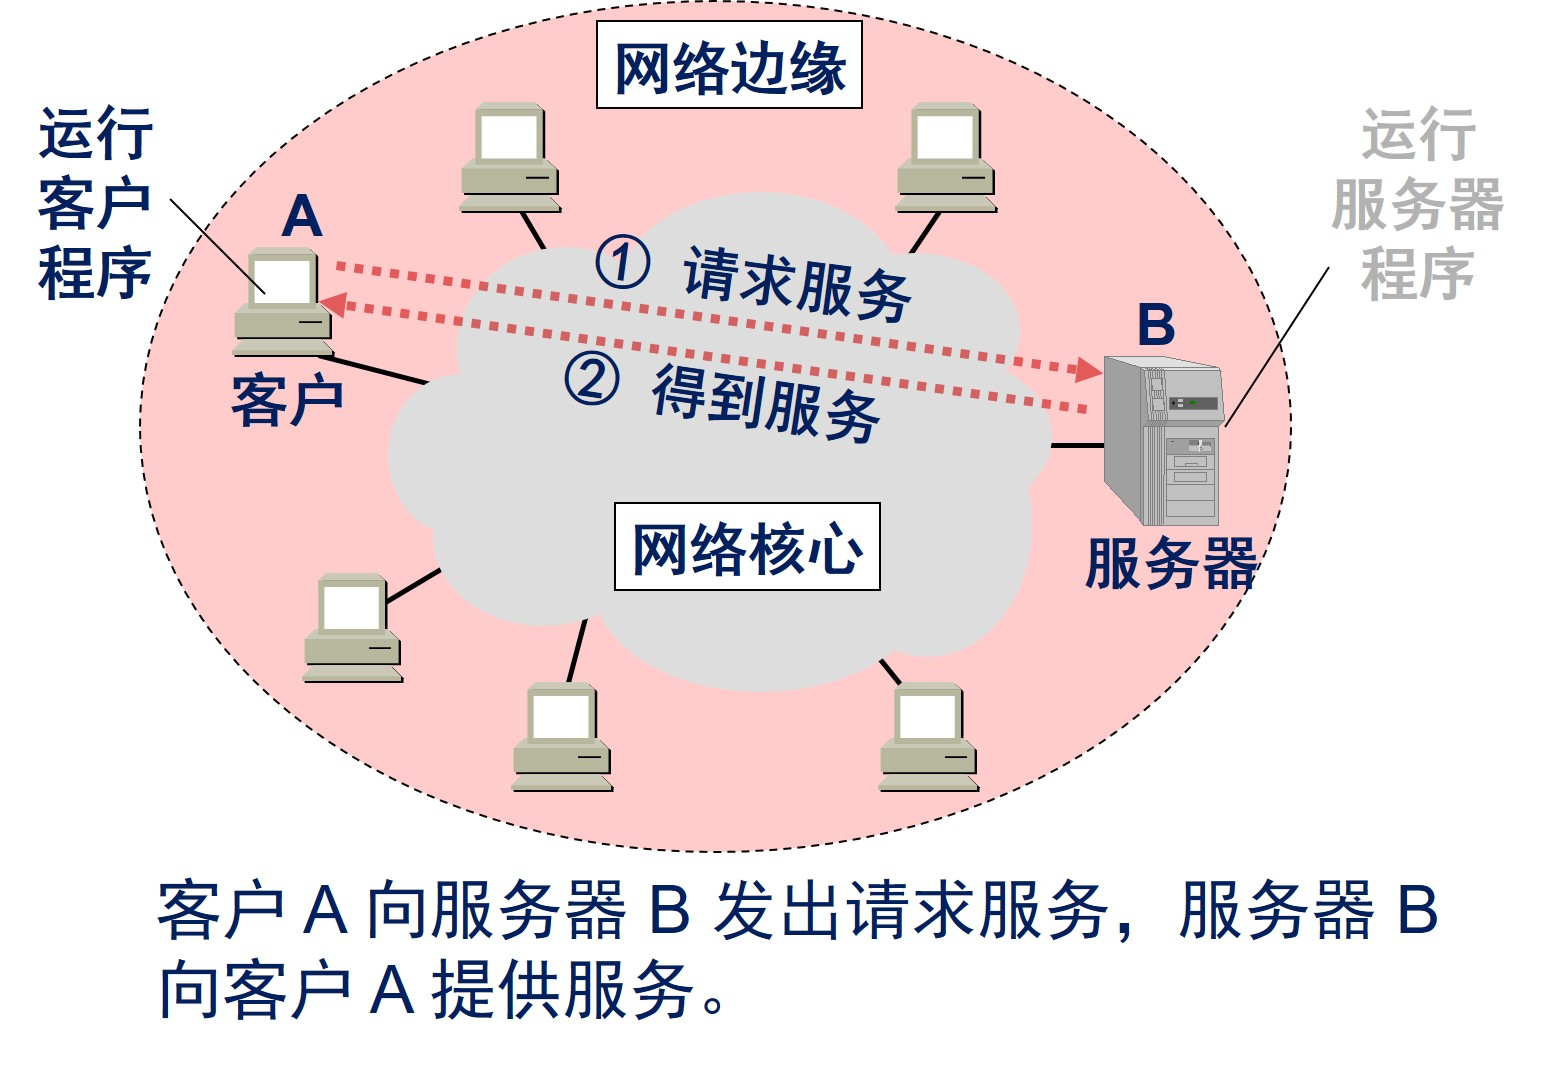
\includegraphics[width=0.4\textwidth]{fig_7_03}(a)
  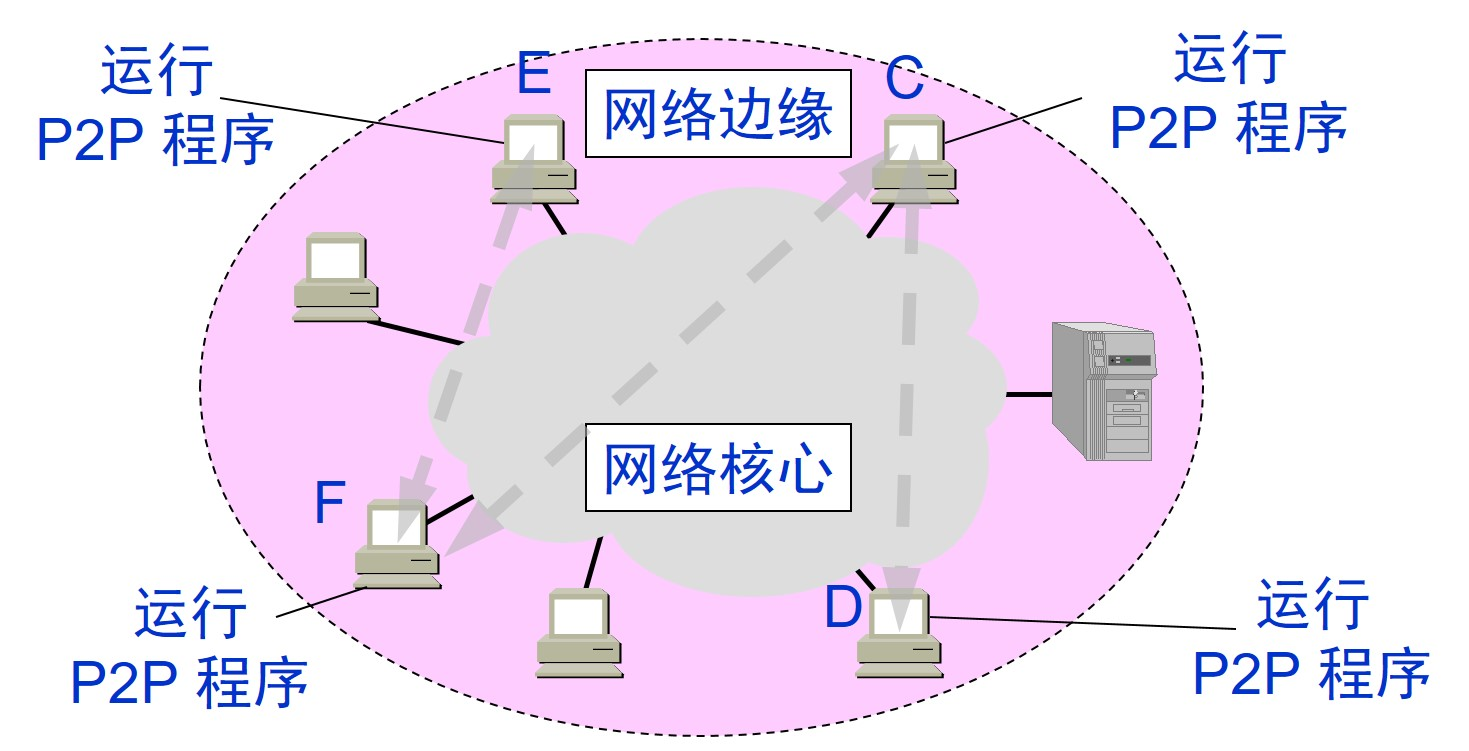
\includegraphics[width=0.5\textwidth]{fig_7_03a}(b)\\
  \caption{连接方式. (a)C/S方式,(b)P2P方式。}\label{fig_7_03}
\end{figure}


\subsection{核心部分}
网络中的核心部分要向网络边缘中的大量主机提供连通性,使边缘部分中的任何一个主机都能够向其他主机通信(即传送或接收各种形式的数据)。
在网络核心部分起特殊作用的是路由器(router)。
路由器是实现分组交换(packet switching)的关键构件,其任务是转发收到的分组,这是网络核心部分最重要的功能。


如图\ref{fig_7_04}所示,电路交换是指在通信双方建立一条临时专用线路的过程。两部电话机只需要用一对电线就能够互相连接起来;5 部电话机两两相连,需 10 对电线。N 部电话机两两相连,需 N(N – 1)/2 对电线。当电话机的数量很大时,这种连接方法需要的电线对的数量与电话机数的平方成正比。。

\begin{figure}
  \centering
  % Requires \usepackage{graphicx}
  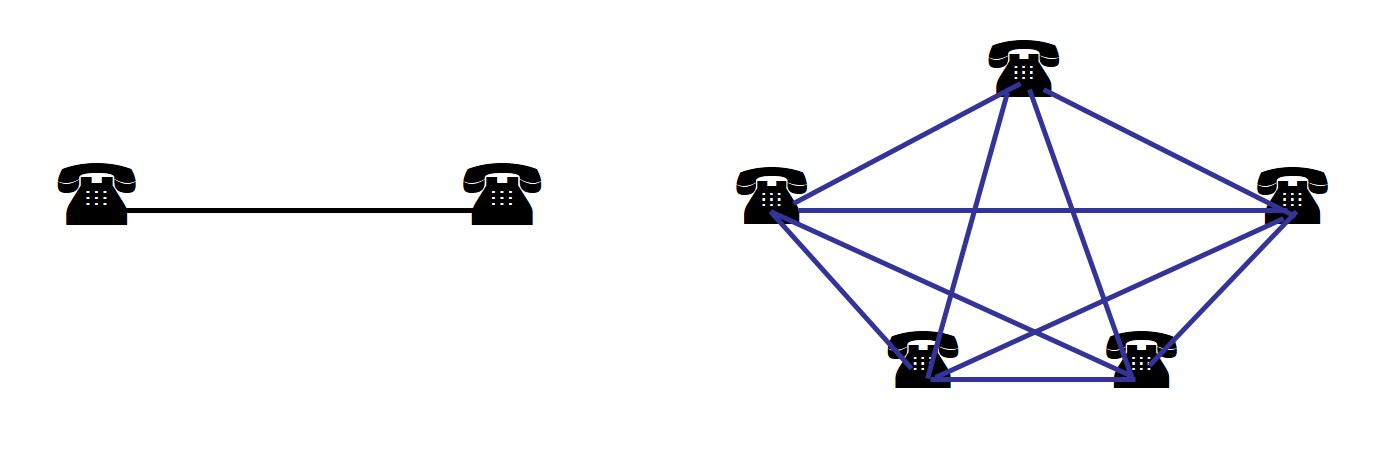
\includegraphics[width=0.5\textwidth]{fig_7_04}
  \caption{电话机互相连通}\label{fig_7_04}
\end{figure}


当电话机的数量增多时,就要使用交换机来完成全网的交换任务,如图\ref{fig_7_05}所示。“交换”(switching)的含义就是转接——把一条电话线转接到另一条电话线,使它们连通起来。从通信资源的分配角度来看,“交换”就是按照某种方式动态分配传输线路的资源。


\begin{figure}
  \centering
  % Requires \usepackage{graphicx}
  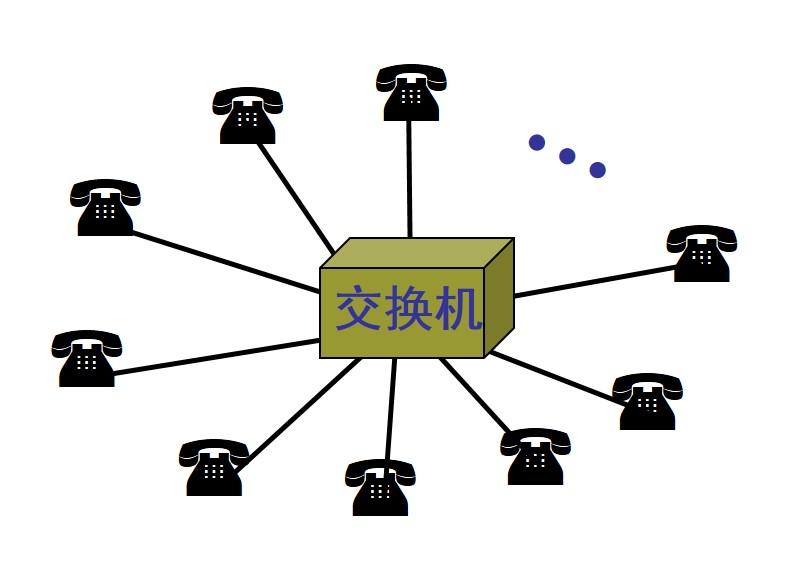
\includegraphics[width=0.3\textwidth]{fig_7_05}
  \caption{交换机}\label{fig_7_05}
\end{figure}

电路交换必定是面向连接的。电路交换的三个阶段:

\begin{enumerate}
          \item 建立连接
          \item 通信
          \item 释放连接
\end{enumerate}


\begin{figure}
  \centering
  % Requires \usepackage{graphicx}
  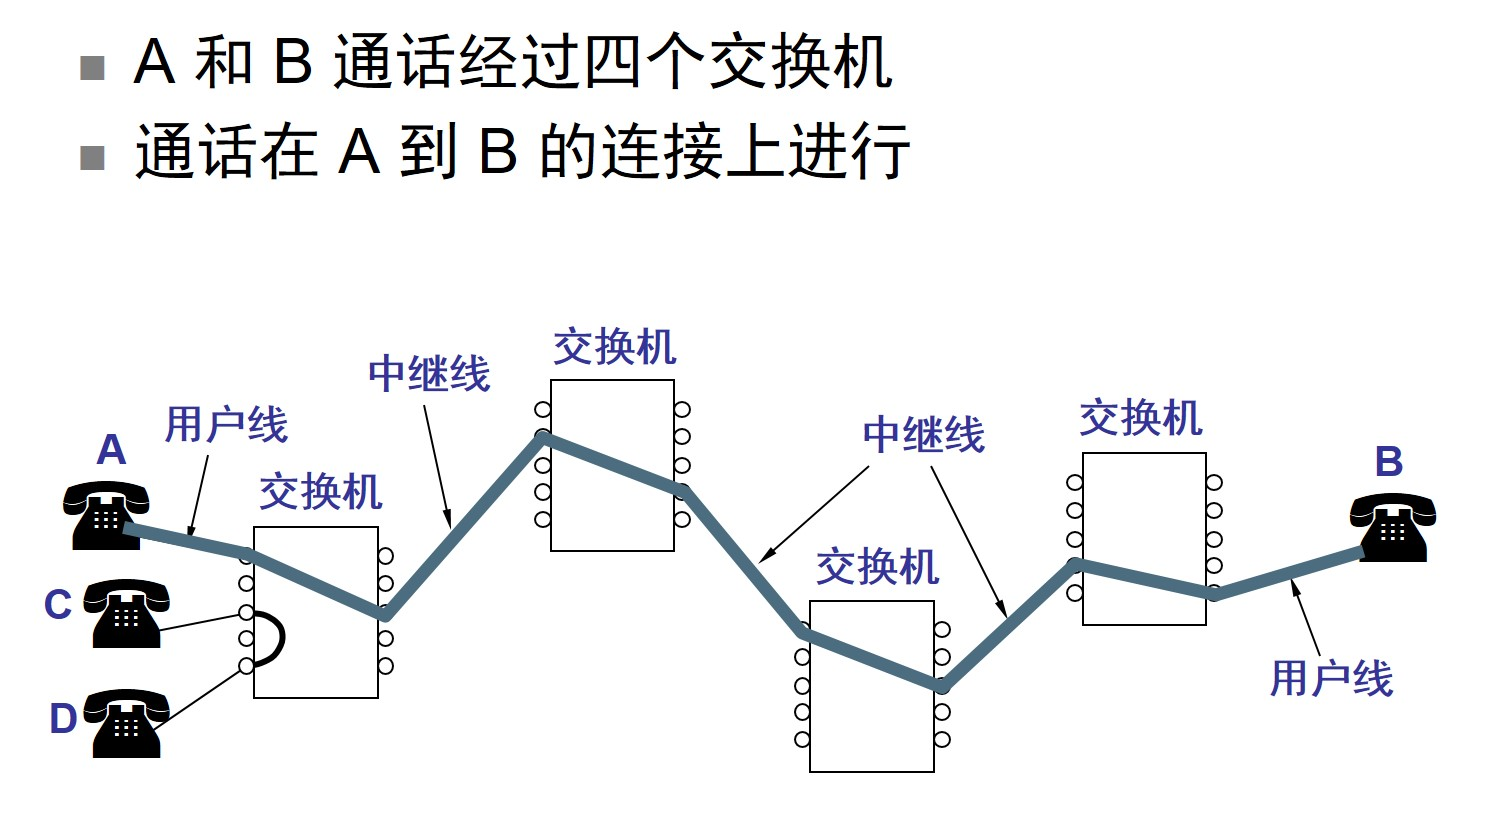
\includegraphics[width=0.6\textwidth]{fig_7_06}
  \caption{电路交换举例}\label{fig_7_06}
\end{figure}


电路交换特点:

\begin{itemize}
  \item 线路建立连接的时间较长(缺点)
  \item 一旦建立连接就独占线路,线路利用率低(缺点)
  \item 建立连接后,数据传输延时小(优点)
\end{itemize}

结论:电路交换不适合计算机通信,因为计算机通信具有突发性的特点,计算机真正传输数据的时间不超过10%。
例如:假定建立连接的时间为0.5秒,计算机以1Mb的速率发送10k字节,此时线路利用率极低。

分组交换的过程:分组交换是以分组为单位,按照存储-转发的方式进行数据传输的,即将到达交换机的分组先送到存储器暂时存储和处理,等到相应的输出线路有空闲时再送出,如图所示。

\begin{enumerate}
  \item 在发送端,先把较长的报文划分成较短的、固定长度的数据段。
  \item 每一个数据段前面添加上首部构成分组。
  \item 分组交换网以“分组”作为数据传输单元。依次把各分组发送到接收端
\item 最后,接收端收到分组后剥去首部,把收到的数据恢复成为原来的报文。

\end{enumerate}


\begin{figure}
  \centering
  % Requires \usepackage{graphicx}
  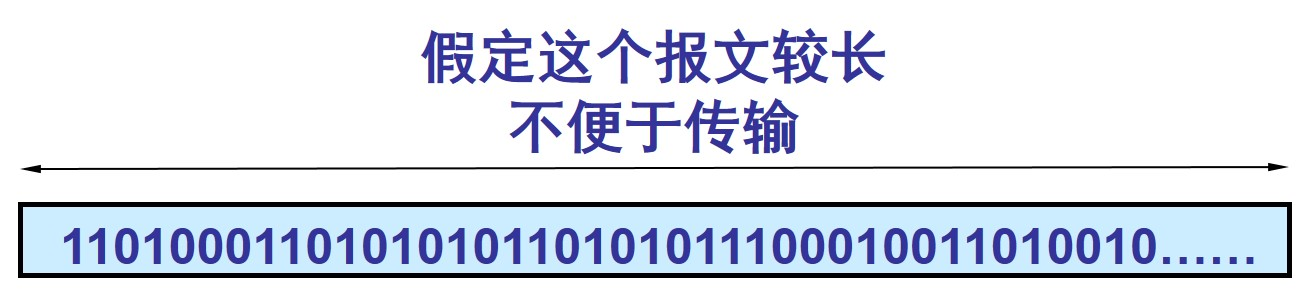
\includegraphics[width=0.4\textwidth]{fig_7_07}\\(a)待发送数据\\
  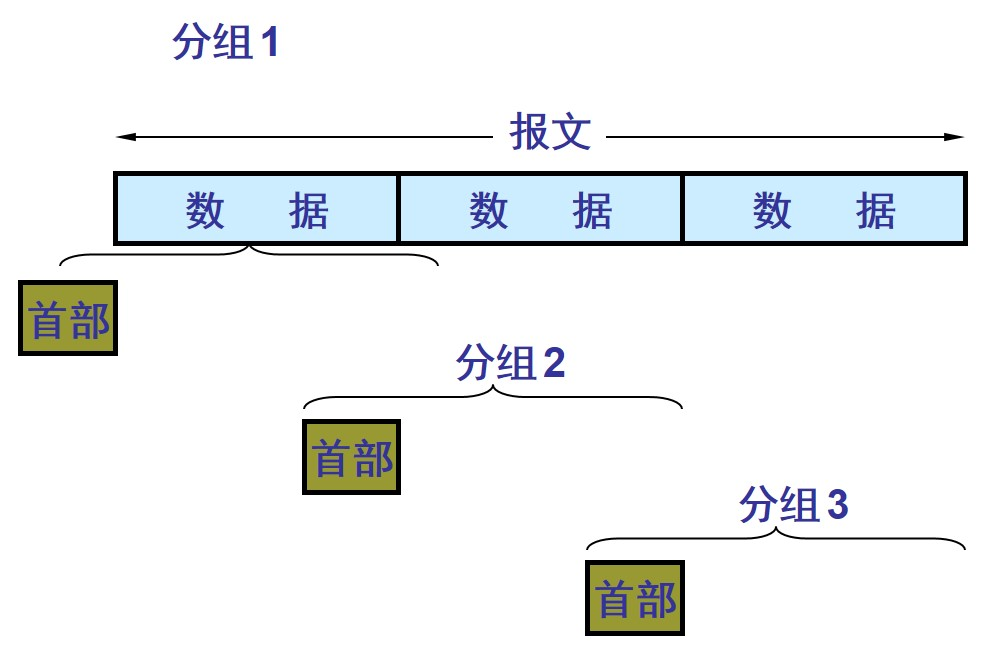
\includegraphics[width=0.4\textwidth]{fig_7_07a}\\(b) 添加首部\\
  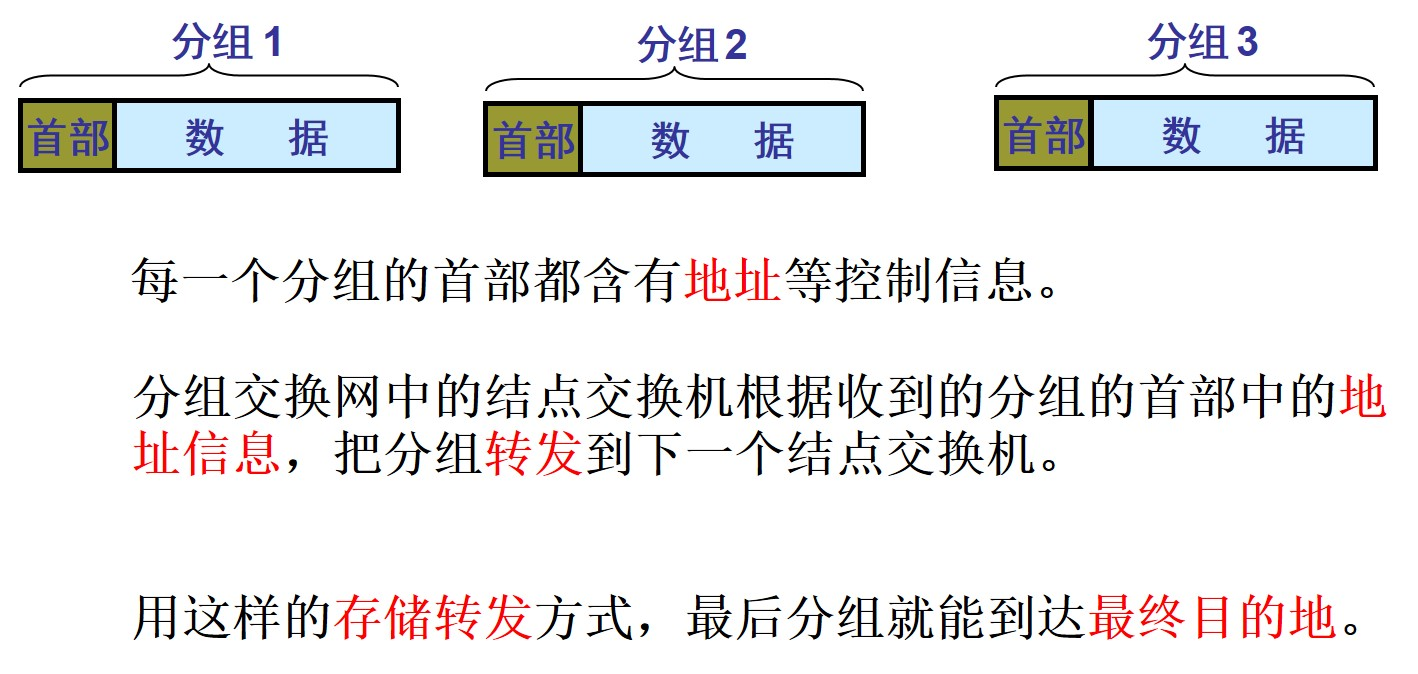
\includegraphics[width=0.4\textwidth]{fig_7_07b}\\(c) 分组传输\\
  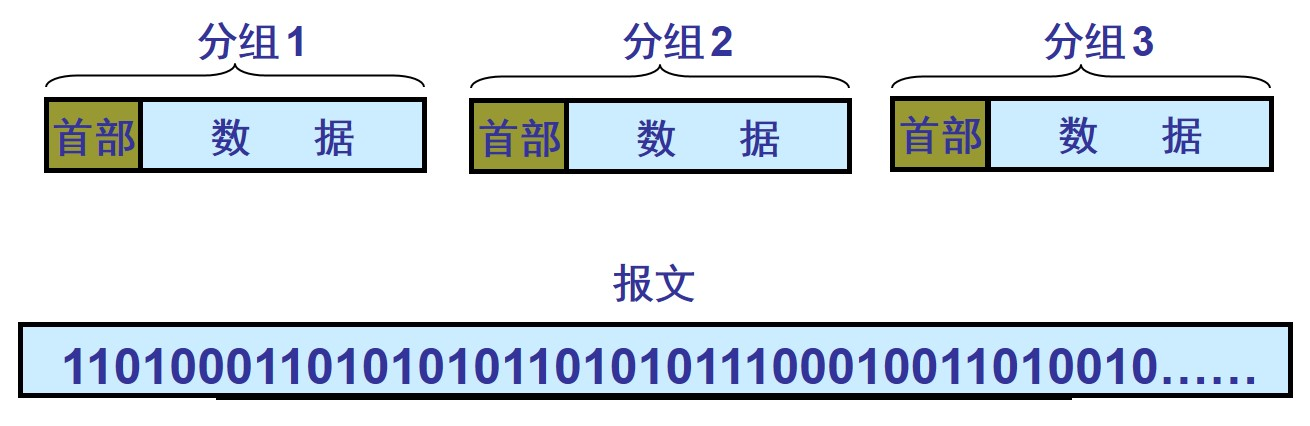
\includegraphics[width=0.4\textwidth]{fig_7_07c}\\(d) 报文还原\\
  \caption{分组交换的过程 }\label{fig_7_07}
\end{figure}


路由器处理分组过程:
\begin{enumerate}
  \item 把收到的分组先放入缓存(暂时存储);

  \item 查找转发表,根据数据中的目的地址,确定应从哪个端口转发;

  \item 把分组送到适当的端口转发出去。

\end{enumerate}

分组交换的优点:

\begin{description}
  \item[高效] 动态分配传输带宽,对通信链路是逐段占用。

  \item[灵活] 为每一分组独立地选择转发路由。

  \item[迅速] 不必先建立连接就能向其他主机发送分组。

  \item[可靠] 保证可靠性的网络协议;分布式的路由选择协议使网络有很好的生存性。

\end{description}

分组交换的缺点:
\begin{itemize}
  \item 分组在各结点存储转发时需要排队,这就会造成一定的时延。


  \item 分组必须携带的首部(里面有必不可少的控制信息)也造成了一定的开销。

\end{itemize}

\begin{figure}
  \centering
  % Requires \usepackage{graphicx}
  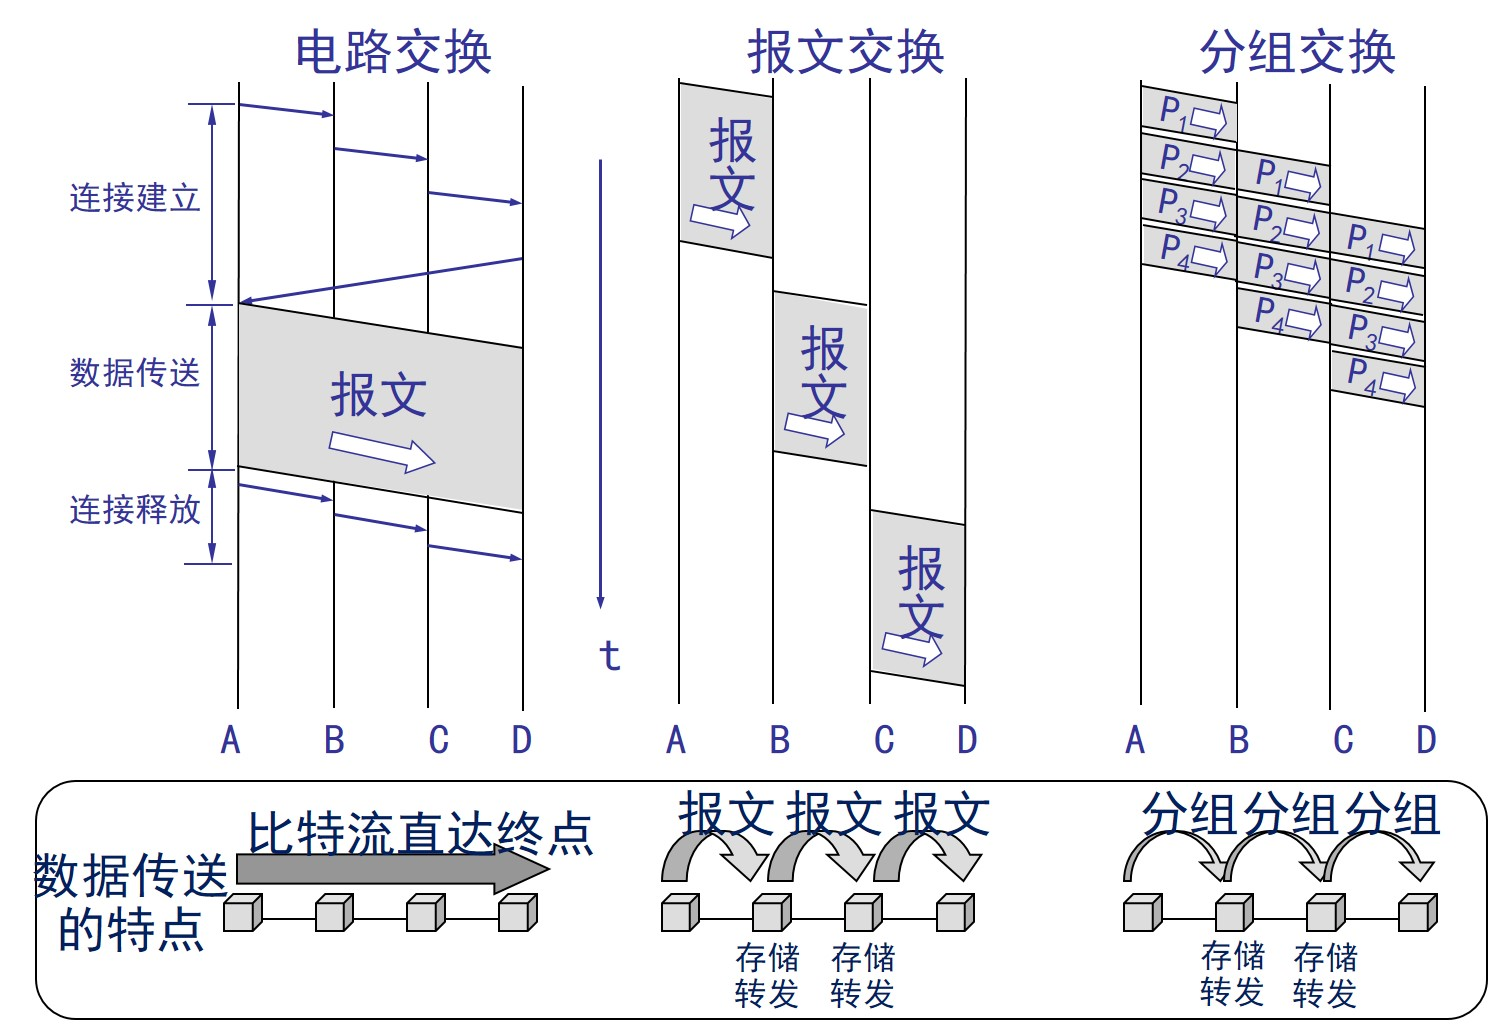
\includegraphics[width=0.6\textwidth]{fig_7_08}
  \caption{电路交换、报文交换、分组交换}\label{fig_7_08}
\end{figure}



\subsection{计算机网络的类别}

不同作用范围的网络:
\begin{itemize}
  \item 个人区域网 PAN (Personal Area Network)

  \item 局域网 LAN (Local Area Network)

  \item 城域网 MAN (Metropolitan Area Network)

  \item 广域网 WAN (Wide Area Network)

\end{itemize}

从网络的使用者进行分类

\begin{itemize}
  \item 公用网 (public network)

  \item 专用网 (private network)

\end{itemize}


\subsection{计算机网络的性能}

\subsubsection{速率}

\textbf{速率}即数据率(data rate)或比特率(bit rate)是计算机网络中最重要的一个性能指标。速率的单位是 b/s,或kb/s, Mb/s, Gb/s 等速率往往是指额定速率或标称速率。

\subsubsection{带宽}
\textbf{带宽(bandwidth)}本来是指信号具有的频带宽度,单位是赫(或千赫、兆赫、吉赫等)。现在“带宽”是数字信道所能传送的“最高数据率”的同义语,单位是“比特每秒”,或 b/s (bit/s)。

\begin{remark}
常用的带宽单位是

千比每秒,即 kb/s

兆比每秒,即 Mb/s

吉比每秒,即 Gb/s

太比每秒,即 Tb/s

$1k = 2^{10} = 1024$, $1M = 2^{20}$, $1G = 2^{30}$, $1T = 2^{40}$。
\end{remark}


\subsubsection{吞吐量}
\textbf{吞吐量(throughput)}表示在单位时间内通过某个网络(或信道、接口)的数据量。
吞吐量更经常地用于对现实世界中的网络的一种测量,以便知道实际上到底有多少数据量能够通过网络。
吞吐量受网络的带宽或网络的额定速率的限制。

\subsubsection{时延(delay 或 latency)}


\begin{description}
  \item[传输时延(发送时延 )] 发送数据时,数据块从结点进入到传输媒体所需要的时间。也就是从发送数据帧的第一个比特算起,到该帧的最后一个比特发送完毕所需的时间。
  \item[传播时延] 电磁波在信道中需要传播一定的距离而花费的时间。 信号传输速率(即发送速率)和信号在信道上的传播速率是完全不同的概念。
  \item[处理时延] 交换结点为存储转发而进行一些必要的处理所花费的时间
  \item[排队时延] 结点缓存队列中分组排队所经历的时延。排队时延的长短往往取决于网络中当时的通信量。

\end{description}

\textbf{总时延 = 发送时延+传播时延+处理时延+排队时延}

\begin{figure}
  \centering
  % Requires \usepackage{graphicx}
  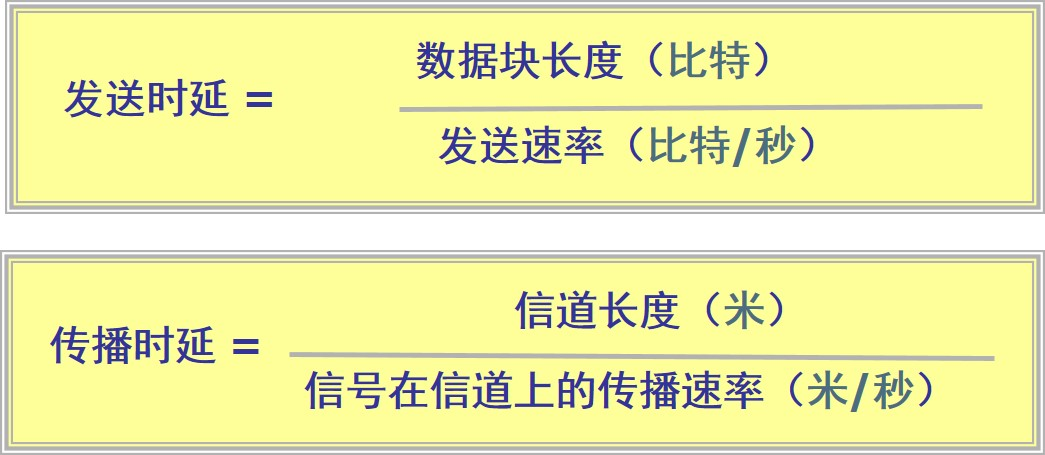
\includegraphics[width=0.4\textwidth]{fig_7_09}
  \caption{传输时延(发送时延 )与传播时延}\label{fig_7_09}
\end{figure}

\begin{figure}
  \centering
  % Requires \usepackage{graphicx}
  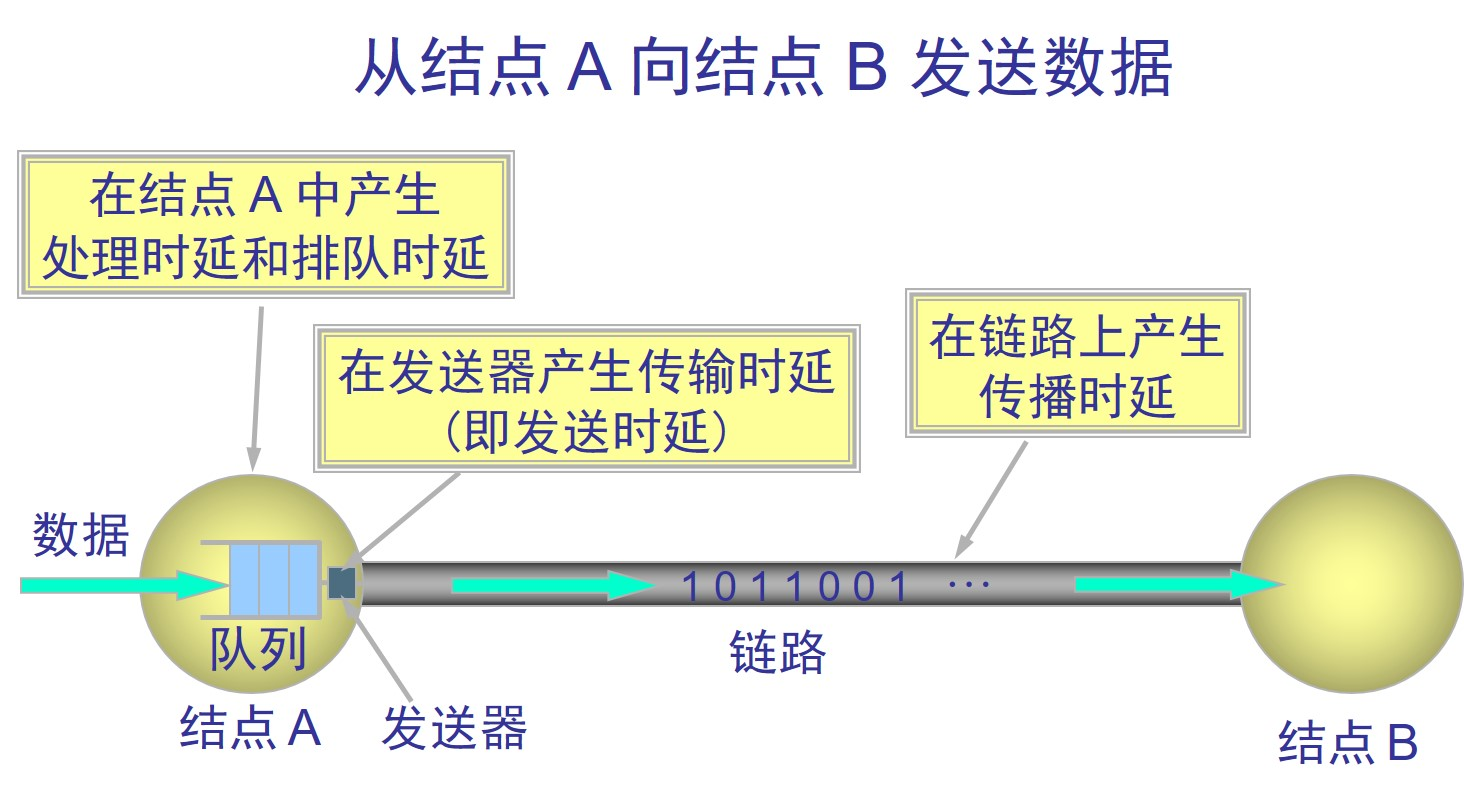
\includegraphics[width=0.6\textwidth]{fig_7_09a}
  \caption{四种时延所产生的地方}\label{fig_7_09a}
\end{figure}


\subsubsection{时延带宽积}

链路的时延带宽积又称为以比特为单位的链路长度,如图\ref{fig_7_10}所示。
\begin{figure}
  \centering
  % Requires \usepackage{graphicx}
  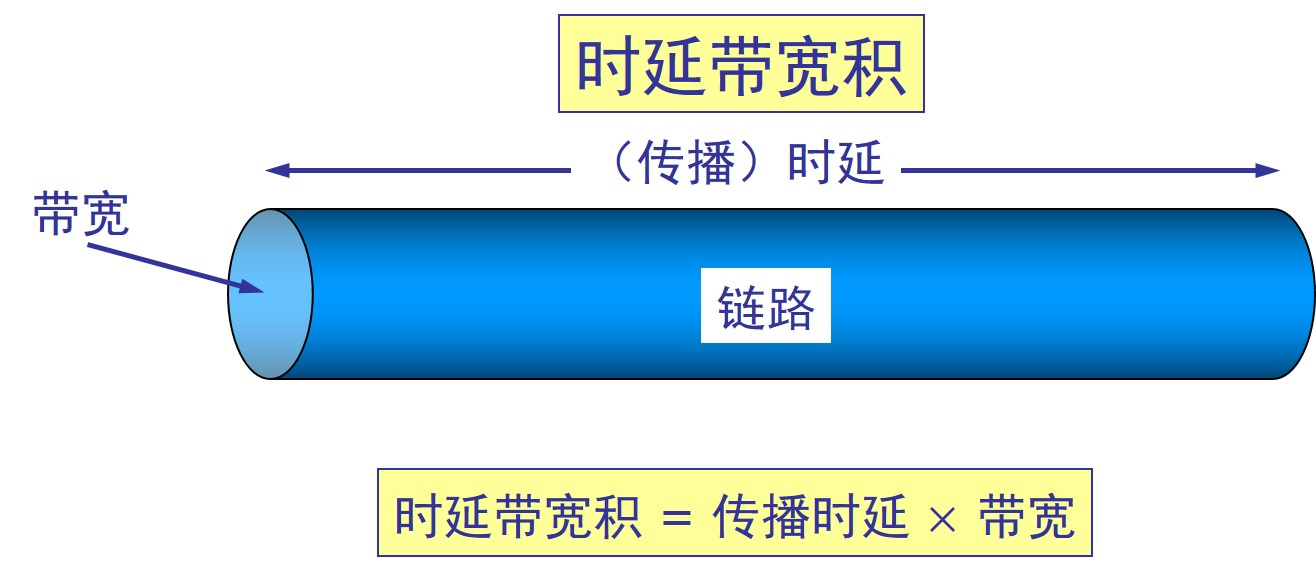
\includegraphics[width=0.5\textwidth]{fig_7_10}
  \caption{时延带宽积}\label{fig_7_10}
\end{figure}

\subsubsection{利用率}
利用率指出某信道有百分之几的时间是被利用的(有数据通过)。完全空闲的信道的利用率是零。
网络利用率则是全网络的信道利用率的加权平均值。
信道利用率并非越高越好。
\begin{figure}
  \centering
  % Requires \usepackage{graphicx}
  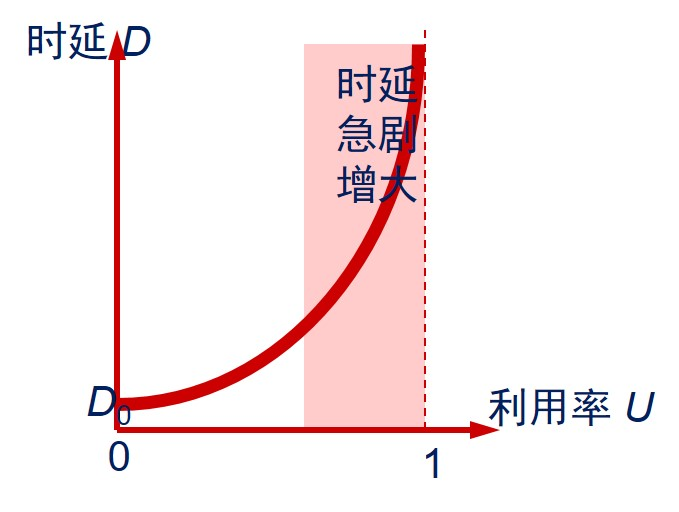
\includegraphics[width=0.3\textwidth]{fig_7_11}
  \caption{时延与利用率的关系}\label{fig_7_11}
\end{figure}



\section{计算机网络体系结构}


\subsection{体系结构的形成}


相比于传统的邮政通信系统,计算机之间相互通信涉及到许多复杂的技术问题,而解决这一复杂问题十分有效的方法是分层解决。
采用层次结构的目的是使各厂家在研制计算机网络系统时由一个共同遵守的标准。


\subsection{OSI体系结构}

计算机网络体系结构基本概念
\begin{description}
  \item[实体] 在网络分层体系结构中,每一层都由一些实体组成。在一个计算机系统中,任何可发送或接收信息的硬件或软件进程都可成为一个实体。
  \item[层次]通常将系统中能提供某种或某类型服务功能的逻辑构造称为一个层次
  \item[协议] 是指两个对等实体间完成通信或服务所必须遵循的规则和约定。网络协议主要由以下三个要素组成:
  \begin{enumerate}
    \item 语法。规定如何进行通信,即对通信双方采用的数据格式、编码等进行定义。

    \item 语义。规定用于协调双方动作的信息及其含义,它是发出的命令请求、完成的动作和返回的响应组成的集合,即对发出的请求、执行的动作以及对方的应答做出解释。

    \item 时序。规定事件实现顺序的详细说明,即确定通信状态的变化和过程,例如通信双方的应答关系、是采用同步传输还是异步传输等。

  \end{enumerate}
由此可见:计算机网络体系结构是实体、层次、协议的集合,是计算机网络及其部件所应完成功能的精确定义。

\end{description}


计算机网络系统采用层次化网络体系结构具有以下优点:

\begin{itemize}
  \item 易促进标准化工作

  \item 各层之间相互独立

  \item 易于实现和维护
\item 灵活性好

\end{itemize}




\begin{figure}
  \centering
  % Requires \usepackage{graphicx}
  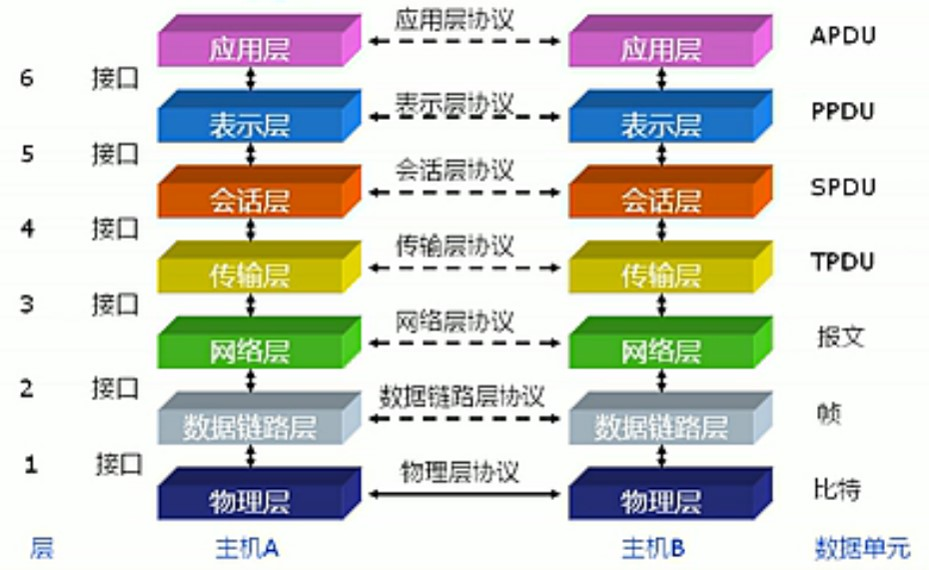
\includegraphics[width=0.6\textwidth]{fig_7_12}
  \caption{开放系统互连OSI模型}\label{fig_7_12}
\end{figure}


\subsection{TCP/IP体系结构}

通信系统只要遵循 OSI 标准,一个系统就可以和位于世界上任何地方的、也遵循这同一标准的其他任何系统进行通信。

然而OSI标准在市场化方面 却失败了:

\begin{itemize}
  \item OSI 的协议实现起来过分复杂,且运行效率很低;

  \item OSI 标准的制定周期太长;

  \item OSI 的层次划分并也不太合理,有些功能在多个层次中重复出现。

\end{itemize}

法律上的国际标准 OSI 并没有得到市场的认可。非国际标准 TCP/IP 现在获得了最广泛的应用。TCP/IP 常被称为事实上的国际标准。
TCP/IP协议的起源:美国国防部高级研究计划局(ARPA)从20世纪60年代开始致力于研究不同类型计算机网络之间的相互联接问题,并成功开发出了著名的传输控制协议/网际协议(TCP/IP)协议。TCP/IP协议是将计算机组成网络的一系列协议的总和,其命名源于其中最重要的两个协议,一个是TCP(Transmission Control Protocol)协议,称为传输控制协议,另一个是IP(Internet Protocol)协议。

\begin{itemize}
  \item 应用层(application layer)

  \item 运输层(transport layer)

  \item 网络层(network layer)

  \item 数据链路层(data link layer)

  \item 物理层(physical layer)

\end{itemize}

\begin{remark}
  TCP/IP体系结构有时也用四层表示方法,即用网络接口层代替数据链路层和物理层。

\end{remark}

\section{计算机网络协议}


\subsection{物理层}
物理层的主要任务描述为确定与传输媒体的接口的一些特性,即:


\begin{description}
  \item[机械特性] 指明接口所用接线器的形状和尺寸、引线数目和排列、固定和锁定装置等等。
  \item[电气特性] 指明在接口电缆的各条线上出现的电压的范围。

  \item[功能特性] 指明某条线上出现的某一电平的电压表示何种意义。
  \item[过程特性] 指明对于不同功能的各种可能事件的出现顺序。
\end{description}


\begin{figure}
  \centering
  % Requires \usepackage{graphicx}
  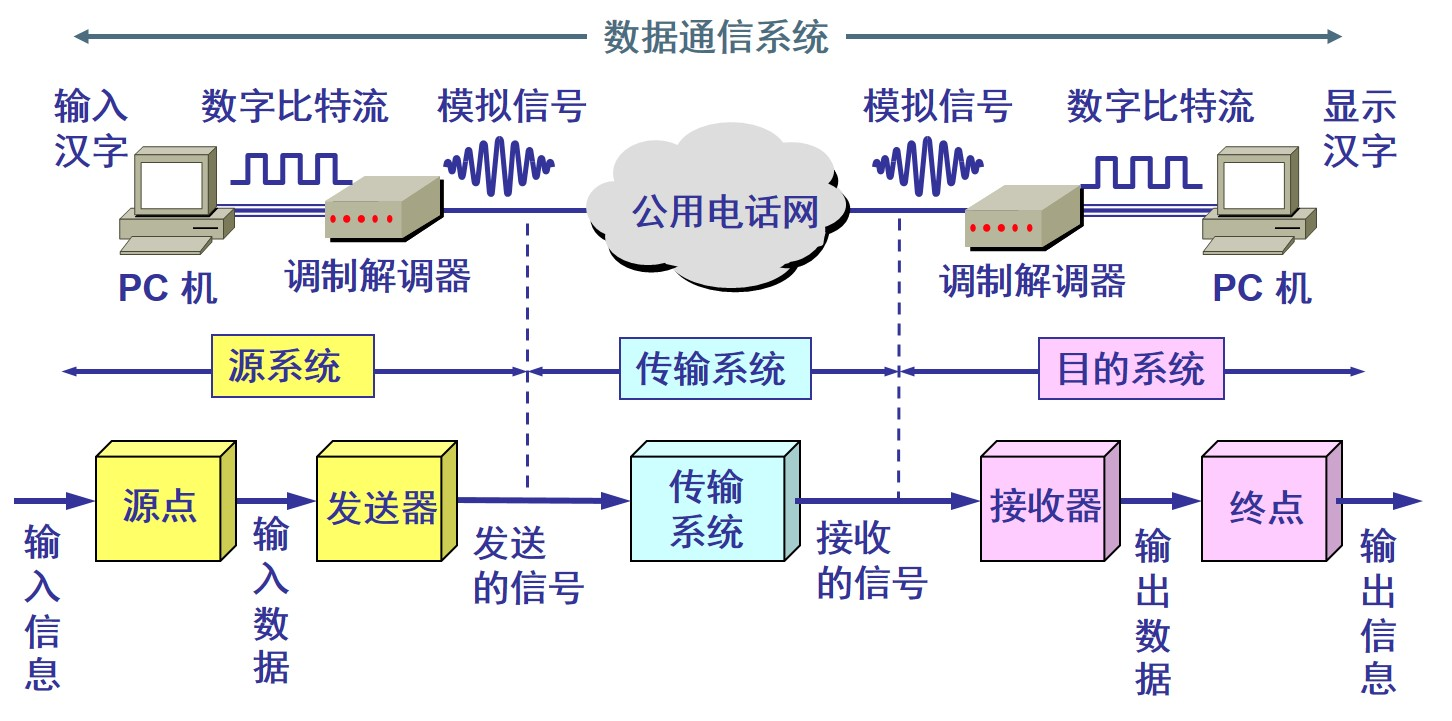
\includegraphics[width=0.6\textwidth]{fig_7_13}\\
  \caption{数据通信系统的模型}\label{fig_7_13}
\end{figure}


\begin{figure}
  \centering
  % Requires \usepackage{graphicx}
  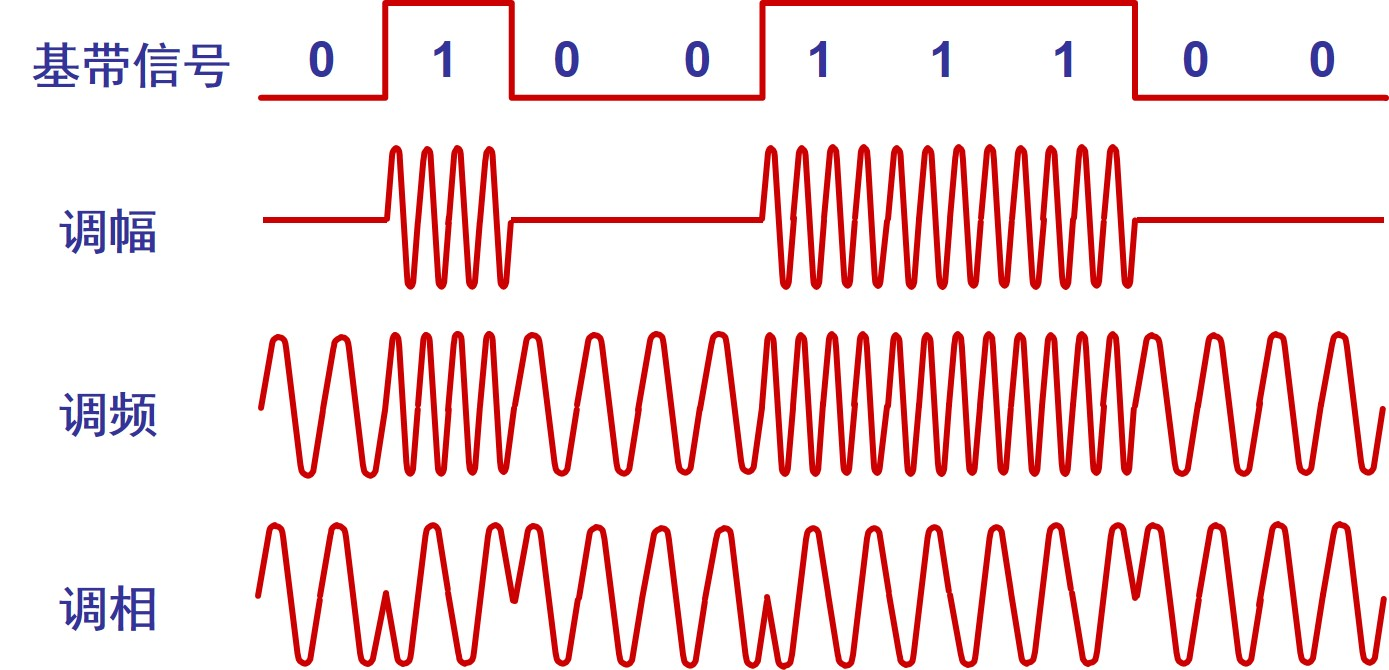
\includegraphics[width=0.5\textwidth]{fig_7_14}\\
  \caption{对基带数字信号的几种调制方法 }\label{fig_7_14}
\end{figure}



\begin{figure}
  \centering
  % Requires \usepackage{graphicx}
  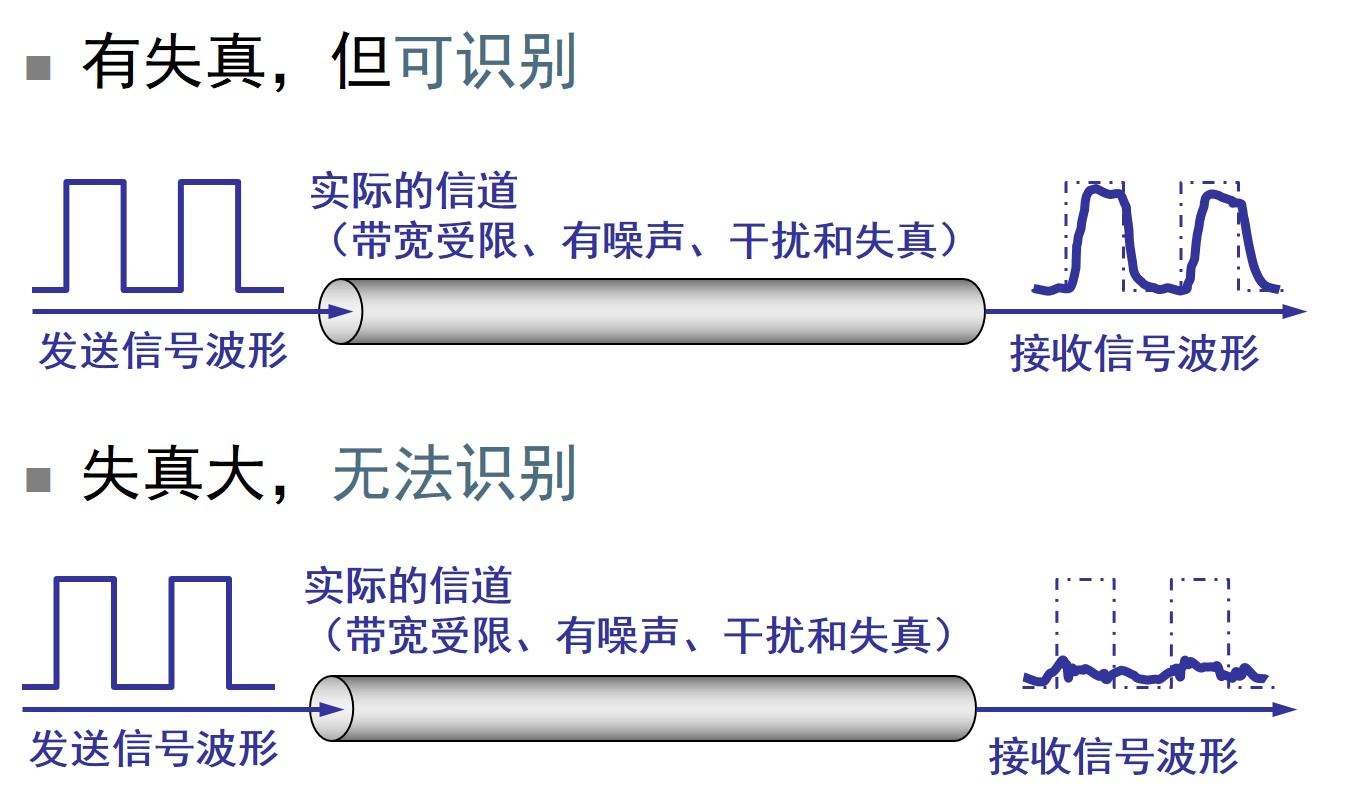
\includegraphics[width=0.5\textwidth]{fig_7_15}\\
  \caption{数字信号通过实际的信道 }\label{fig_7_15}
\end{figure}



信道复用技术:复用(multiplexing)是通信技术中的基本概念。
频分复用、时分复用和统计时分复用等。

\begin{description}
  \item[频分复用(Frequency Division Multiplexing) ]用户在分配到一定的频带后,在通信过程中自始至终都占用这个频带。
频分复用的所有用户在同样的时间占用不同的带宽资源(请注意,这里的“带宽”是频率带宽而不是数据的发送速率)。

  \item[时分复用(Time Division Multiplexing)]时分复用则是将时间划分为一段段等长的时分复用帧(TDM 帧)。每一个时分复用的用户在每一个 TDM 帧中占用固定序号的时隙。
每一个用户所占用的时隙是周期性地出现(其周期就是 TDM  帧的长度)。
TDM 信号也称为等时(isochronous)信号。
时分复用的所有用户是在不同的时间占用同样的频带宽度。

时分复用可能造成线路资源浪费:使用时分复用系统传送计算机数据时,由于计算机数据的突发性质,用户对分配到的子信道的利用率一般是不高的。
  \item[统计时分复用(Statistic TDM)]
  \item[波分复用 (Wavelength Division Multiplexing)] 波分复用就是光的频分复用
  \item[码分复用(Code Division Multiplexing) ]常用的名词是码分多址 CDMA
    (Code Division Multiple Access)。
各用户使用经过特殊挑选的不同码型,因此彼此不会造成干扰。
这种系统发送的信号有很强的抗干扰能力,其频谱类似于白噪声,不易被敌人发现。
每一个比特时间划分为 m 个短的间隔,称为码片(chip)。
\end{description}



\begin{figure}
  \centering
  % Requires \usepackage{graphicx}
  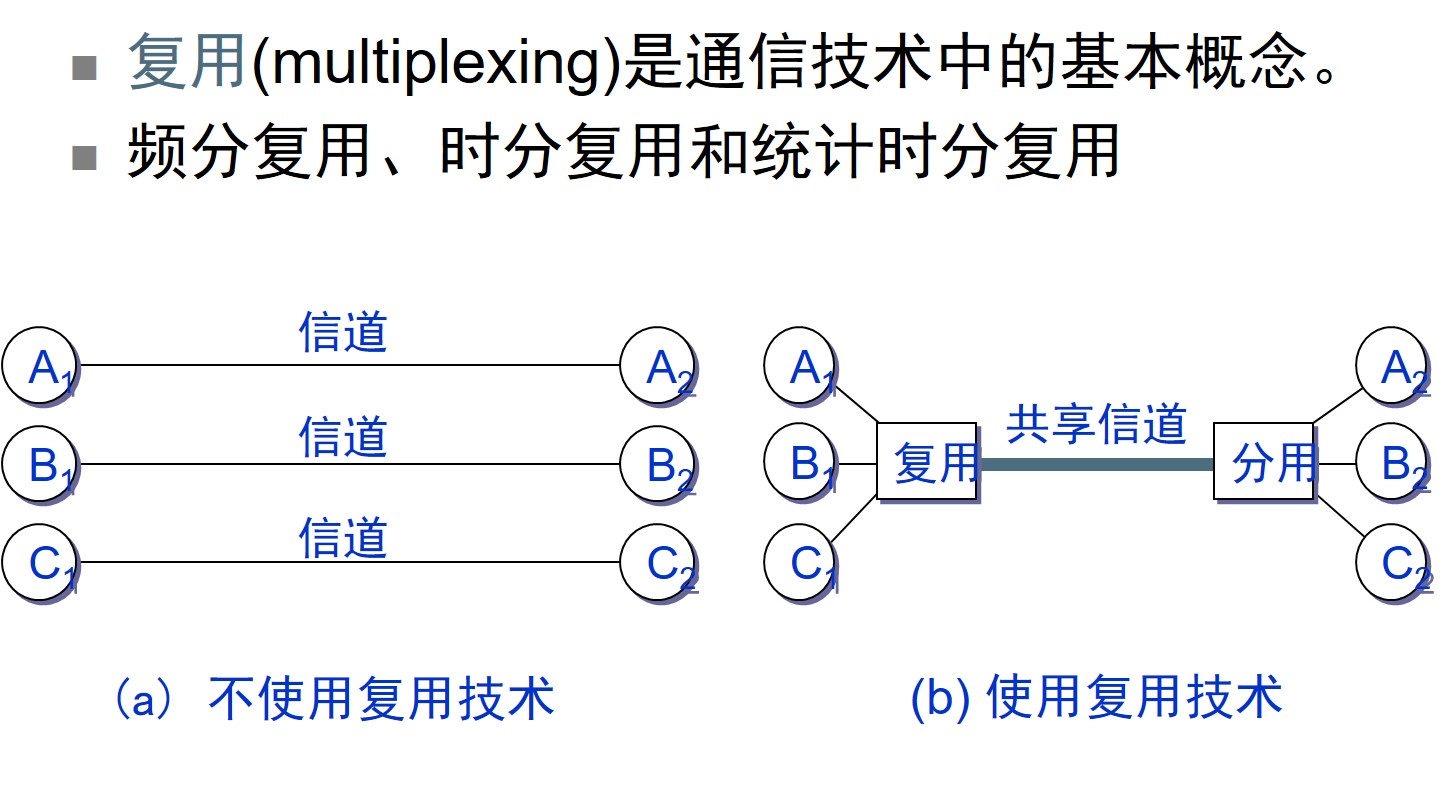
\includegraphics[width=0.5\textwidth]{fig_7_16}\\
  \caption{信道复用技术 }\label{fig_7_16}
\end{figure}









\subsection{数据链路层}

数据链路(data link) 除了物理线路外,还必须有通信协议来控制这些数据的传输。若把实现这些协议的硬件和软件加到链路上,就构成了数据链路。
      \begin{itemize}
        \item 现在最常用的方法是使用适配器(即网卡)来实现这些协议的硬件和软件。

        \item 一般的适配器都包括了数据链路层和物理层这两层的功能。

      \end{itemize}


数据链路层使用的信道主要有以下两种类型:
\begin{itemize}
  \item 点对点信道:这种信道使用一对一的点对点通信方式。

  \item 广播信道:这种信道使用一对多的广播通信方式,因此过程比较复杂。广播信道上连接的主机很多,因此必须使用专用的共享信道协议来协调这些主机的数据发

\end{itemize}


常常在两个对等的数据链路层之间画出一个数字管道,而在这条数字管道上传输的数据单位是帧。早期的数据通信协议曾叫作通信规程(procedure)。 因此在数据链路层,规程和协议是同义语。





\begin{figure}
  \centering
  % Requires \usepackage{graphicx}
  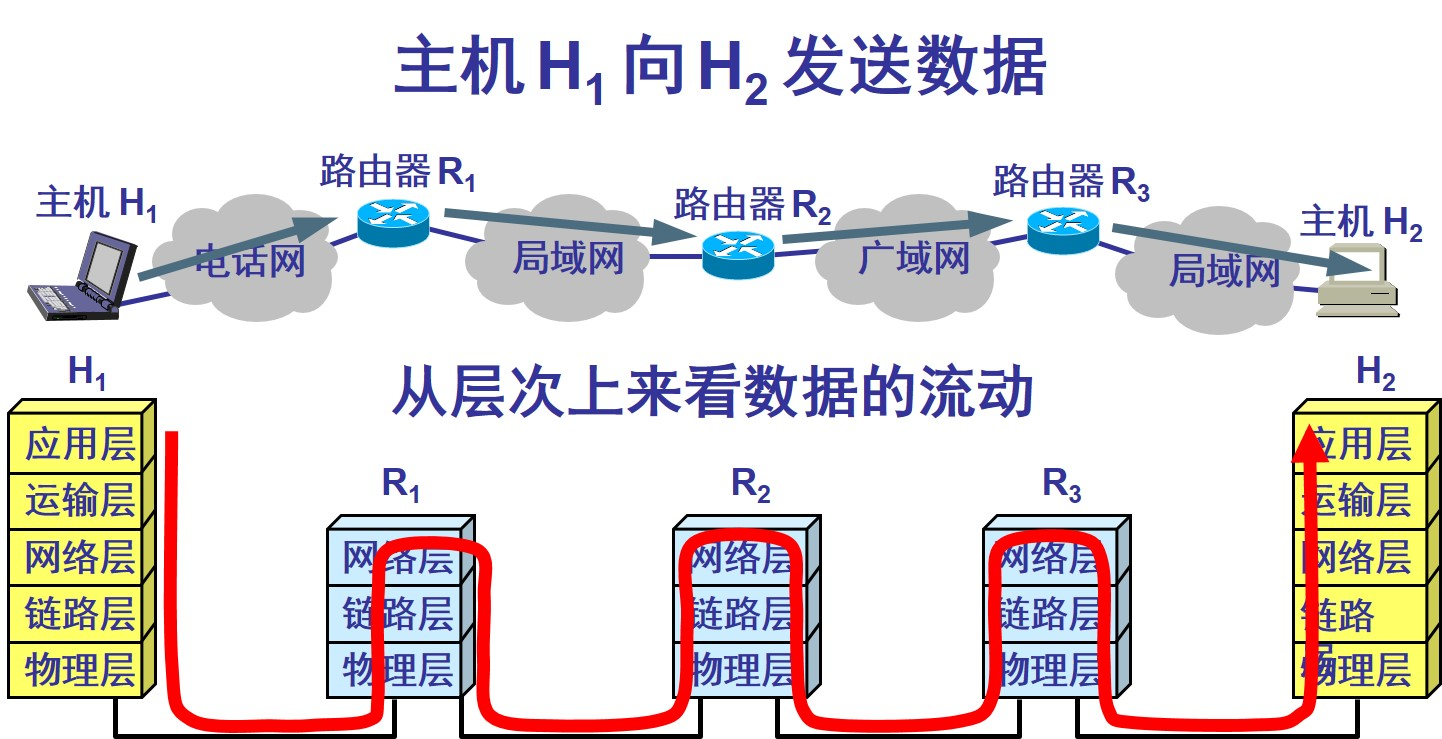
\includegraphics[width=0.6\textwidth]{fig_7_17}\\
  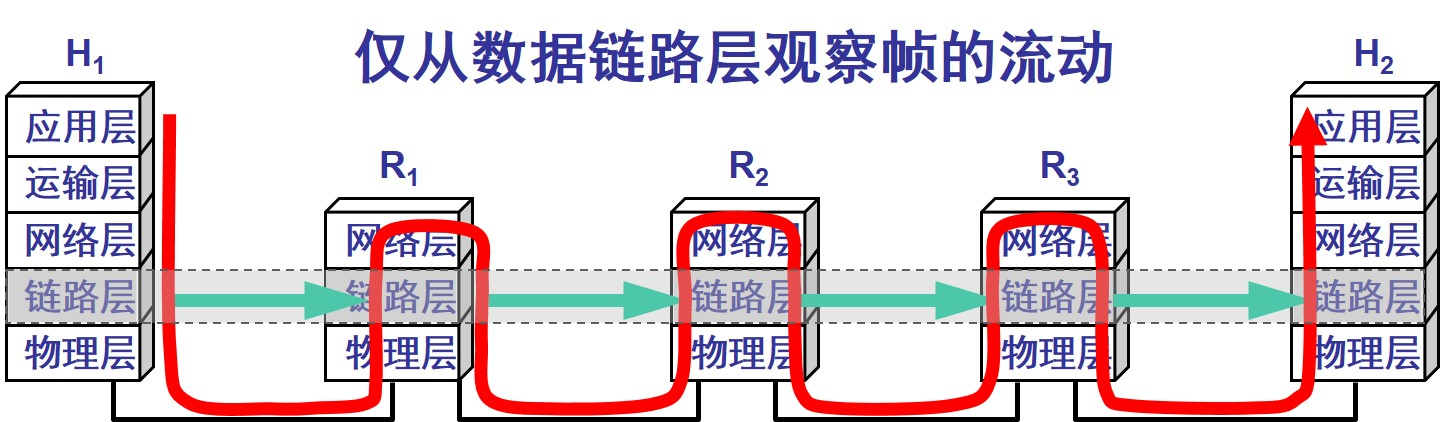
\includegraphics[width=0.6\textwidth]{fig_7_17a}\\
  \caption{数据链路层的简单模型 }\label{fig_7_17}
\end{figure}



\subsection{网络层}

在计算机网络领域,网络层应该向运输层提供怎样的服务(“面向连接”还是“无连接”)曾引起了长期的争论。
争论焦点的实质就是:在计算机通信中,可靠交付应当由谁来负责?是网络还是端系统?

\begin{itemize}
  \item 电信网络:由网络负责可靠交付

\begin{itemize}
  \item 面向连接的通信方式

  \item 建立虚电路(Virtual Circuit),以保证双方通信所需的一切网络资源。

  \item 如果再使用可靠传输的网络协议,就可使所发送的分组无差错按序到达终点。

\end{itemize}





\begin{remark}
虚电路表示这只是一条逻辑上的连接,分组都沿着这条逻辑连接按照存储转发方式传送,而并不是真正建立了一条物理连接。
请注意,电路交换的电话通信是先建立了一条真正的连接。因此分组交换的虚连接和电路交换的连接只是类似,但并不完全一样。
\end{remark}




  \item 网络层:不提供质量服务保证,尽最大努力交付
\begin{itemize}
  \item 网络层向上只提供简单灵活的、无连接的、尽最大努力交付的数据报服务。

  \item 网络在发送分组时不需要先建立连接。每一个分组(即 IP 数据报)独立发送,与其前后的分组无关(不进行编号)。

  \item 网络层不提供服务质量的承诺。即所传送的分组可能出错、丢失、重复和失序(不按序到达终点),当然也不保证分组传送的时限。

  \item 由于传输网络不提供端到端的可靠传输服务,这就使网络中的路由器可以做得比较简单,而且价格低廉(与电信网的交换机相比较)。

  \item 如果主机(即端系统)中的进程之间的通信需要是可靠的,那么就由网络的主机中的运输层负责(包括差错处理、流量控制等)。

  \item  采用这种设计思路的好处是:网络的造价大大降低,运行方式灵活,能够适应多种应用。

\end{itemize}


\end{itemize}





\subsection{运输层}

运输层向应用层提供通信服务,
它属于面向通信部分的最高层,同时也是用户功能中的最低层。
运输层为应用进程之间提供端到端的逻辑通信(但网络层是为主机之间提供逻辑通信)。
运输层还要对收到的报文进行差错检测。
运输层需要有两种不同的运输协议,即面向连接的 TCP 和无连接的 UDP。

TCP/IP 的运输层有两个不同的协议:

\begin{enumerate}
  \item 用户数据报协议 UDP(User Datagram Protocol)

UDP 在传送数据之前不需要先建立连接。对方的运输层在收到UDP报文后,不需要给出任何确认。虽然 UDP 不提供可靠交付,但在某些情况下UDP是一种最有效的工作方式。



  \item 传输控制协议 TCP(Transmission Control Protocol)

TCP则提供面向连接的服务。TCP不提供广播或多播服务。由于TCP要提供可靠的、面向连接的运输服务,因此不可避免地增加了许多的开销。这不仅使协议数据单元的首部增大很多,还要占用许多的处理机资源。

\end{enumerate}




运输层的端口:

运行在计算机中的进程是用进程标识符来标志的。
运行在应用层的各种应用进程却不应当让计算机操作系统指派它的进程标识符。这是因为在因特网上使用的计算机的操作系统种类很多,而不同的操作系统又使用不同格式的进程标识符。
为了使运行不同操作系统的计算机的应用进程能够互相通信,就必须用统一的方法对 TCP/IP 体系的应用进程进行标志。
解决这个问题的方法就是在运输层使用协议端口号(protocol port number),或通常简称为端口(port)。
虽然通信的终点是应用进程,但我们可以把端口想象是通信的终点,因为我们只要把要传送的报文交到目的主机的某一个合适的目的端口,剩下的工作(即最后交付目的进程)就由 TCP 来完成。



\subsection{应用层}

应用层协议的特点:每个应用层协议都是为了解决某一类应用问题,而问题的解决又往往是通过位于不同主机中的多个应用进程之间的通信和协同工作来完成的。应用层的具体内容就是规定应用进程在通信时所遵循的协议。
应用层的许多协议都是基于客户服务器方式。客户(client)和服务器(server)都是指通信中所涉及的两个应用进程。客户服务器方式所描述的是进程之间服务和被服务的关系。客户是服务请求方,服务器是服务提供方。

\begin{enumerate}
  \item 域名系统 DNS

许多应用层软件经常直接使用域名系统 DNS (Domain Name System),但计算机的用户只是间接而不是直接使用域名系统。
因特网采用层次结构的命名树作为主机的名字,并使用分布式的域名系统 DNS。
名字到 IP 地址的解析是由若干个域名服务器程序完成的。域名服务器程序在专设的结点上运行,运行该程序的机器称为域名服务器。

  \item 文件传送协议 FTP

  文件传送协议 FTP (File Transfer Protocol) 是因特网上使用得最广泛的文件传送协议。
FTP 提供交互式的访问,允许客户指明文件的类型与格式,并允许文件具有存取权限。
FTP 屏蔽了各计算机系统的细节,因而适合于在异构网络中任意计算机之间传送文件。
RFC 959 很早就成为了因特网的正式标准。


  \item 远程终端协议 TELNET

  TELNET 是一个简单的远程终端协议,也是因特网的正式标准。
用户用 TELNET 就可在其所在地通过 TCP 连接注册(即登录)到远地的另一个主机上(使用主机名或 IP 地址)。
TELNET 能将用户的击键传到远地主机,同时也能将远地主机的输出通过 TCP 连接返回到用户屏幕。这种服务是透明的,因为用户感觉到好像键盘和显示器是直接连在远地主机上。


  \item 万维网 WWW

  万维网 WWW (World Wide Web)并非某种特殊的计算机网络。
万维网是一个大规模的、联机式的信息储藏所。
万维网用链接的方法能非常方便地从因特网上的一个站点访问另一个站点,从而主动地按需获取丰富的信息。
这种访问方式称为“链接”。


\end{enumerate}





\section{无线与移动网络}


\subsection{无线网络概述}
无线局域网基本概念:就是利用无线电波作为信息传输的媒介构成的无线局域网(WLAN),与有线网络的用途十分类似,最大的不同在于传输媒介的不同,利用无线电技术取代网线。
无线网络的分类,如图\ref{fig_7_18}所示。

\begin{figure}
  \centering
  % Requires \usepackage{graphicx}
  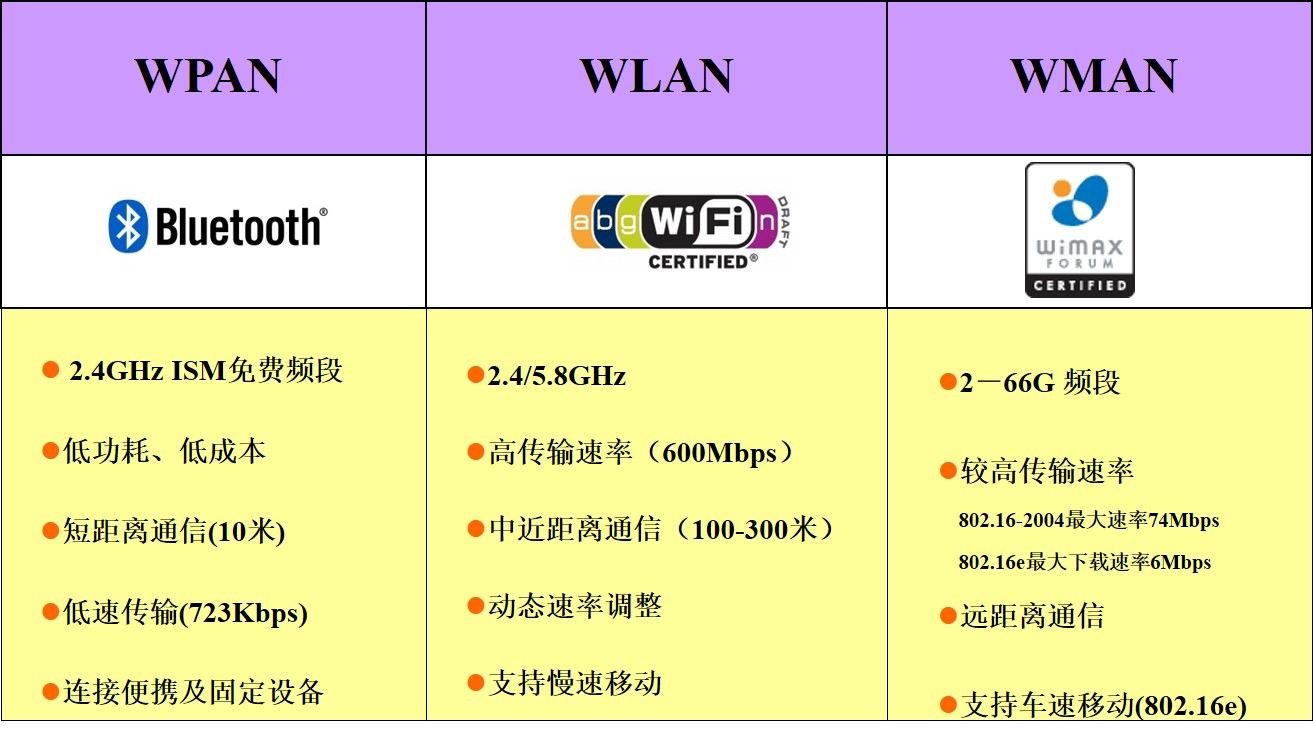
\includegraphics[width=0.65\textwidth]{fig_7_18}
  \caption{无线网络分类}\label{fig_7_18}
\end{figure}


无线网常用的实现技术有:IEEE的802.11系列协议族、家用射频工作组提出的HomeRF、Bluetooth,及3G技术等。
该课程主要讨论以IEEE 802.11协议为基础的无线局域网我们常说的“WLAN”指的就是符合802.11系列协议的无线局域网技术


\begin{itemize}
  \item 802.11
  \item 802.11b
  \item 802.11a
  \item 802.11g
  \item 802.11n
\end{itemize}



\subsection{无线局域网的组网}

\begin{itemize}
  \item 
有固定基础设施无线局域网特点


\begin{itemize}
  \item 
有中心拓扑,又被称为集中控制式
  \item 每一个单元由一个中心站控制,网中的终端在该中心站的控制下与其他终端通信
  \item 对中心站的依赖性较高,抗毁性差
  \item 随着网络中用户的增多,中心站的负担将加重;

\end{itemize}
  \item 
无固定基础设施的无线局域网-Ad Hoc

\begin{itemize}
  \item 
所有移动站点都处于平等地位
  \item 无中心站,所有站点之间可直接进行通信
  \item 所有站点之间共享一条信道
  \item 用户增加时,冲突非常厉害,适用于用户少且范围小的组网;

\end{itemize}

\end{itemize}
\subsection{无线局域网的标准}

无线局域网的标准如图\ref{fig_7_19}所示。


\begin{figure}
  \centering
  % Requires \usepackage{graphicx}
  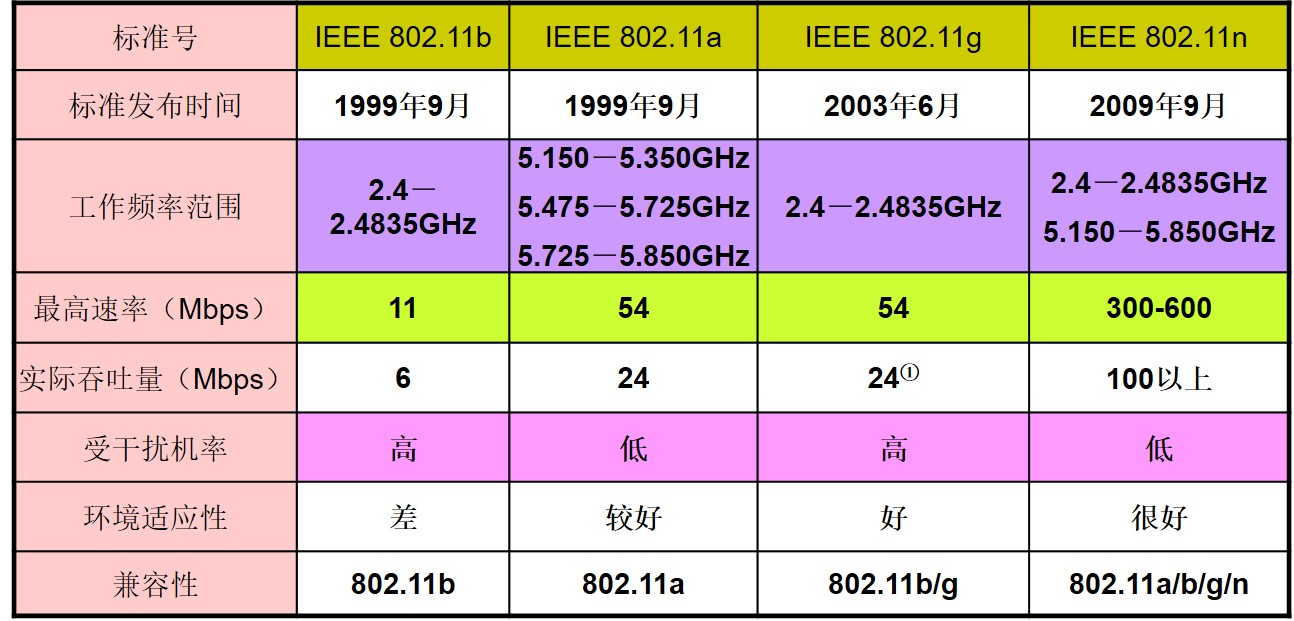
\includegraphics[width=0.65\textwidth]{fig_7_19}
  \caption{无线局域网的标准}\label{fig_7_19}
\end{figure}

\subsection{无线局域网的传输方式}
数据在无线局域网进行传输通常有以下几种实现方法:

\subsubsection{(1)红外线方式}
目前,广泛使用的家电遥控器几乎都是采用红外线传输技术。作为无线局域网的传输方式,红外线的最大优点是不受无线电干扰,且红外线的使用不受国家无线电管理委员会的限制。然而,红外线对非透明物体的透过性极差,这导致传输距离受限。

\subsubsection{(2)窄带调制方式}
在窄带调制方式中,数据基带信号的频谱不做任何扩展即被直接搬移到射频发射出去。
与扩展频谱方式相比,窄带调制方式占用频带少、频带利用率高但带来的问题是,当临近的仪器设备或通信设备也在使用这一频段时,会严重影响通信质量,通信的可靠性无法得到保障。

\subsubsection{(3)扩展频谱方式}
在扩展频谱方式中,数据基带信号的频谱被扩展至几倍甚至几十倍后再被搬移至射频发射出去。
这一做法虽然牺牲了频带带宽,却提高了通信系统的抗干扰能力和安全性。由于单位频带内的功率降低,对其他电子设备的干扰也减小了。


\subsection{无线局域网基本特性}




\section{网上多媒体应用、网络安全}



\subsection{网络安全问题概述}
计算机网络面临的安全性威胁
\begin{itemize}
  \item 计算机网络上的通信面临以下的四种威胁:
  \begin{enumerate}
    \item 截获——从网络上窃听他人的通信内容。
    \item 中断——有意中断他人在网络上的通信。
    \item 篡改——故意篡改网络上传送的报文。
    \item 伪造——伪造信息在网络上传送。
  \end{enumerate}
  \item 截获信息的攻击称为被动攻击,而更改信息和拒绝用户使用资源的攻击称为主动攻击。

\end{itemize}



\subsection{两类密码体制}

\subsubsection{对称密钥密码体制}

所谓常规密钥密码体制,即加密密钥与解密密钥是相同的密码体制。
这种加密系统又称为对称密钥系统。

\subsubsection{公钥密码体制}

公钥密码体制使用不同的加密密钥与解密密钥,是一种“由已知加密密钥推导出解密密钥在计算上是不可行的”密码体制。

公钥密码体制的产生主要是因为两个方面的原因,一是由于常规密钥密码体制的密钥分配问题,另一是由于对数字签名的需求。

现有最著名的公钥密码体制是RSA 体制,它基于数论中大数分解问题的体制,由美国三位科学家 Rivest, Shamir 和 Adleman 于 1976 年提出并在 1978 年正式发表的。


\subsection{数字签名}


数字签名必须保证以下三点:

\begin{enumerate}
  \item 报文鉴别——接收者通过报文中的签名能够核实发送者的身份;
  \item 报文的完整性——接受到的数据应与发送完全一样,未被篡改过;
  \item 不可否认——发送者不能否认发送过的签名文件。
\end{enumerate}

现在已有多种实现各种数字签名的方法。但采用公钥算法更容易实现。


\subsection{防火墙}

防火墙是由软件、硬件构成的系统,是一种特殊编程的路由器,用来在两个网络之间实施接入控制策略。接入控制策略是由使用防火墙的单位自行制订的,为的是可以最适合本单位的需要。
防火墙内的网络称为“可信赖的网络”(trusted network),而将外部的因特网称为“不可信赖的网络”(untrusted network)。
防火墙可用来解决内联网和外联网的安全问题。


防火墙的功能有两个:阻止和允许。

\begin{itemize}
  \item “阻止”就是阻止某种类型的通信量通过防火墙(从外部网络到内部网络,或反过来)。

  \item “允许”的功能与“阻止”恰好相反。

\end{itemize}




防火墙必须能够识别通信量的各种类型。不过在大多数情况下防火墙的主要功能是“阻止”。
防火墙技术一般分为两类


\begin{enumerate}
  \item 网络级防火墙——用来防止整个网络出现外来非法的入侵。属于这类的有分组过滤和授权服务器。前者检查所有流入本网络的信息,然后拒绝不符合事先制订好的一套准则的数据,而后者则是检查用户的登录是否合法。

  \item 应用级防火墙——从应用程序来进行接入控制。通常使用应用网关或代理服务器来区分各种应用。例如,可以只允许通过访问万维网的应用,而阻止 FTP 应用的通过。

\end{enumerate}

